\documentclass[11pt]{article}
\usepackage{amsmath}
\usepackage{graphicx}
\usepackage{color}
\usepackage{longtable}
\usepackage{tabu}
\usepackage{hyperref}
\usepackage{geometry}
\geometry{left=1.5cm,right=1.5cm,top=1.5cm,bottom=1.5cm}
\usepackage{amsmath}
\usepackage{amssymb}
\usepackage{calc}
\usepackage{ifthen}
\usepackage{tikz}
\usepackage{svg}
\usepackage{float}
\usepackage[backend=bibtex,sorting=none]{biblatex}
\addbibresource{seedom-whitepaper.bib}
\renewcommand*\rmdefault{ppl}
\setlength{\fboxsep}{10pt}
\setlength{\fboxrule}{0.5pt}
\setlength{\parindent}{0pt}

\begin{document}

\title{%
\begin{center}
\includegraphics[width=0.7\textwidth]{../seedom-assets/logo/full/seedom-full-black-transparent.pdf}
\end{center}
\large Seeding the Future of Philanthropy \\[5mm]
\large A Unique FUNdraiser for Causes and Their Supporters \\[5mm]}
\author{Team Palm Tree}
\date{\today}
\maketitle

\begin{abstract}

Have you been to a local raffle that supports a cause at some point in your life? At this kind of fundraising event, you have a room full with eager supporters, representatives from the cause, administrators with rolls of paper tickets with distinct numbers on them, and a set of prizes off in the corner. As the administrators walk around with buckets, they distribute sets of tickets in exchange for the local currency, while retaining a duplicate ticket for each number. Everyone in the room can see these transactions as they occur, giving the audience trust over the process. Administrators, after making their rounds, now combine the buckets of ticket duplicates into one bucket in front of the crowd, drawing a ticket at random for each prize. It is a fascinatingly simple and effective fundraising process.\\\\
Seedom is a fun Ethereum decentralized application (DAPP) for raising awareness and Ether for altruistic causes while rewarding a single participant for their contribution and support. It takes the efficiency, security, and transparency of the traditional single-room raffle and re-invents it with trustlessness and crowd-sourced selection into an entirely new type of fundraiser that scales to the entire world. Bimonthly or roughly every two weeks, a new altruistic cause is chosen, with the help of the community, to receive the majority of funds raised through our smart contract. Most of the remaining portion will go to one of the supporters through a selection process crowd-sourced by the participants, the cause, and Seedom. A small percentage will be taken by the Seedom team as an administration fee to continuously improve the platform over time and extensively promote each cause.

\end{abstract}
\pagebreak

\tableofcontents
\pagebreak

\section{Introduction}

Seedom is an Ethereum decentralized application (DAPP) for raising awareness and Ether for altruistic causes while rewarding a single participant for their contribution and support. The selection of a participant is crowd-sourced by the participants, the cause, and Seedom. Ether raised is not tax deductible and will be distributed according to Table \ref{tab:etherSplitPercentages} at the end of the fundraiser. Administration fees cover Seedom expenses in five operational areas.

\begin{itemize}
\item{\textbf{Staff} sustains our small business, marketing, and development team}
\item{\textbf{Legal} 3rd party counsel to protect all forms of private fundraising rights internationally}
\item{\textbf{Auditing} 3rd party security and financial audits as contracts and the organization changes}
\item{\textbf{Infrastructure} temporary systems on our way to full decentralization}
\item{\textbf{Events} physical fundraisers to further support and promote the cause}
\end{itemize}

\begin{table}[H]
\begin{center}
\begin{tabular}{| c | c | c |}
\hline
\textbf{Cause} & \textbf{Participant} & \textbf{Seedom} \\ \hline
60\% & 35\%  & 5\% \\ \hline
\end{tabular}
\caption{Ether split percentages}
\label{tab:etherSplitPercentages}
\end{center}
\end{table}

\subsection{Cause Selection Methodology}

Seedom is a fun and entertaining platform for seeding the future of philanthropy through the identification and funding of altruistic causes that can drive the future of decentralization. Decentralization can take many forms outside of the technical interpretation and the underpinnings of Ethereum. It includes, but is not limited to, the decentralization of power, knowledge, money, ownership, and control to as many people as possible. Seedom provides a funding mechanism for these causes to persist, meet their long-term goals, and decentralize our future.\\\\
Well before a Seedom fundraiser begins, our team will accept suggestions from causes and our global community of participants. Causes can suggest themselves for a future fundraiser to Seedom directly by emailing team@seedom.io. Participants can make future cause suggestions via our polling smart contract, deployed with each Seedom fundraiser. The Seedom team will have the ultimate discretion of cause selection, identifying an organization that is decentralizing, legitimate, active, exacting, and cooperative.

\begin{itemize}
\item{\textbf{Decentralizing} believes in the decentralization of power in all forms}
\item{\textbf{Legitimate} has a capable team with a clear and effective plan of action}
\item{\textbf{Active} is actively working on solving a problem}
\item{\textbf{Exacting} is solving an urgent and ongoing problem}
\item{\textbf{Cooperative} is willing to work with the Seedom team and accept crypto}
\end{itemize}

\subsection{Inherent Advantages}

Seedom is the first fundraiser and rewards platform with all of the following qualities.

\begin{itemize}
\item{\textbf{Philanthropic} a new cause will be chosen bimonthly}
\item{\textbf{Trustless} trust in the cause is the only requirement}
\item{\textbf{Transparent} all contract transactions publicly visible and immutable}
\item{\textbf{Relevant} our team works with legitimate and focused causes benefiting those with an ongoing need for assistance}
\item{\textbf{Secure} security provided by the Ethereum platform itself}
\item{\textbf{Governed} a polling contract allows participants to suggest future causes to support}
\item{\textbf{Anonymous} your personal information is not required}
\item{\textbf{Private} your information is never revealed}
\item{\textbf{Inclusive} anyone in the world can participate}
\item{\textbf{Affordable} everyone will be able to afford an entry}
\item{\textbf{Limitless} there is no limit to the number of obtainable entries}
\item{\textbf{Instantaneous} payout allocation to the cause and selected participant is immediate}
\end{itemize}

\subsection{Trustlessness}

The Seedom community relies on our team to choose causes twice a month with the help of participants. After deployment, a user requires no trust in our team or the cause, who are only responsible for administering the begin and end the fundraiser. Users, Seedom, and the cause cannot operate outside of the strict rules of the smart contracts and no Ether stored in these contracts can be extracted before the end of a fundraiser, unless canceled.\\\\
The cause and our team have the right to cancel a fundraiser before the end time, which will refund all participants. If the cause or our team fail to end the fundraiser promptly after the end time, a cancel() function opens up to the community, again refunding all participants. Once a fundraiser has ended, the fundraiser contract allocates funds to the cause, a selected participant, and our team, allowing these entities to withdraw while prohibiting all forms of cancellation.

\subsection{Comparison to Other Fundraising Methods}

Many methods exist for raising funds for causes. Outside of direct donations, some of the most popular include crowdfunding, matching gifts, drives, sales, auctions, events, lotteries, and raffles. All of these methods lack many of our inherent advantages.

\subsubsection{Crowdfunding}

Crowdfunding is one of the best ways to raise funds for a cause. Unfortunately, most of the popular fundraising platforms are not on Ethereum and therefore receive none of the many benefits native to the platform. When using a centralized system, such as GoFundMe, one is relying on it to move funds from donors to a cause.\\\\
Initially, GoFundMe does not vet fundraisers, relying on fraud prevention specialists to protect their users. Without trustless transaction transparency, it is impossible to know if user contributions ever made it to the cause. Moreover, many crowdfunding companies charge 8\% fees or higher for any donation, which includes a hefty payment processing fee. Being reliant on traditional payment processors, GoFundMe is only available in a handful of counties.

\subsubsection{Matching, Drives, Sales, and Auctions}

Matching, drives, sales, and auctions are also useful fundraising vehicles. Donation matching requires one to work for or know of a company that offers this perk. Donation drives may involve an intermediary that converts non-monetary donations into the monetary type. Sales of items require the overhead of procuring items to sell in addition to the resale activity. Auctions items must be solicited, hopefully for free, and then sold for donation funds.\\\\
Because of the various requirements and overheads involved with each of these techniques, the timeliness and relevancy of the donations are significant concerns; with intermediaries involved, trust and transparency are paramount yet not easily demonstrated. Moreover, all three of these methods also lack global participation capability.

\subsubsection{Events}

Fundraising events are social gatherings that raise funds and awareness for causes. Often overlooked, face to face communication is indispensable to furthering a cause. However, these gathers can get expensive when selecting a venue, hiring temporary staff, providing food, creating informative materials, etc. Seedom adopts this face-to-face approach at the end of each fundraiser in the form of fundraising and volunteering events. At this point, the bulk of the funds are raised and distributed, making this final event valuable, but not necessary to the success of the overall fundraiser.

\subsubsection{Lotteries and Raffles}

Although Seedom is not a lottery and not a raffle, similar organizations exist worldwide, and all of them have administration fees that allow for their existence. In the United States, nearly every state has a lottery, with a national average administration fee of 4.76\% according to the U.S. Census Bureau \cite{3}; however, this does not include commissions paid out to lottery ticket sellers, which equal this same percentage, on average \cite{4}. All expenses considered, 8-10\% of every lottery ticket sold in the U.S. goes towards the lottery process itself and not the winner(s) and beneficiaries.

\subsection{Similar Ethereum Projects}

Alice, Charitychain, Giveth, and Hypergive are experimental Ethereum fundraising DAPPs currently under development. Many of these platforms go beyond fundraising with fund management to control the internal operations of the causes supported. The first three allow donation refunds if the benefiting organization does not meet promised goals by a deadline. Hypergive creates a direct and secure funding connection between donators and homeless and hungry individuals globally. This channel is similar to one employed by an aid program run by the United Nations that delivered funds to 10,000 Syrian refugees using the Ethereum blockchain \cite{6}, with biometric scanners validating fund recipients.\\\\
Seedom is a FUNdraising DAPP that brings routine attention to causes, and it is agnostic to the internal operational methodologies employed by the receiving organization. The organization can maintain their autonomy over their funds outside of Seedom or community control. However, we believe in transparent end-to-end philanthropic benefit delivery systems, and we will work to integrate with any organization or platform that increases a user's understanding of exactly where their donation went. See Section \ref{figure:givethIntegration} for our future plan to integrate with Giveth.

\section{Seedom Explained}

\begin{figure}[H]
\begin{center}
\includegraphics[width=0.4\textwidth]{../seedom-assets/flow/process-vertical-dark.pdf}
\caption{A visual overview of the Seedom fundraiser}
\end{center}
\end{figure}

\subsection{Seedom Deploys Two Contracts}

The Seedom team deploys a new fundraiser for a new cause bimonthly, or roughly every two weeks, on the 1st and 15th of every month. A Seedom fundraiser deployment consists of two new contracts: fundraiser and polling. Thirteen days is the span of the entire timeline due to February's 28 total days during standard years. Seedom will go on break the 13th through the 14th of every month in addition to the 29th until the end of the month. Upon deployment, the Seedom DAPP, located at seedom.io, will be updated accordingly.

\begin{figure}[H]
\begin{center}
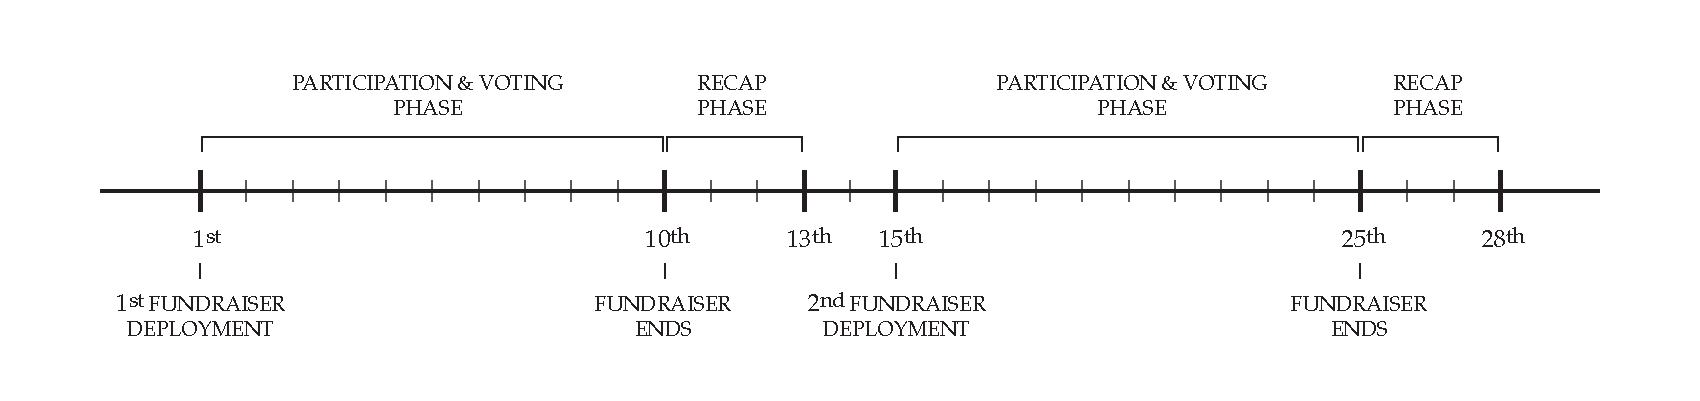
\includegraphics[width=1.0\textwidth]{./graphics/fundraiser-monthly-timeline.pdf}
\caption{Fundraiser monthly timeline}
\label{figure:fundraiserMonthlyTimeline}
\end{center}
\end{figure}

\subsubsection{Fundraiser Contract}

The fundraiser contract deploys with several immutable parameters, including the selected cause, Ether split percentages, Seedom's secret, the cost of an entry, the timing of specific events, and the max number of participants.

\begin{table}[H]
\begin{center}
\begin{tabular}{| l | l | l |}
\hline
\textbf{Parameter} & \textbf{Data Type} & \textbf{Description} \\ \hline
cause & address & the wallet address of the cause \\ \hline
causeSplit & uint256 & the \% of funds given to the cause \\ \hline
participantSplit & uint256 & the \% of funds given to a selected participant \\ \hline
ownerSplit & uint256 & the \% of funds given to the contract owner (Seedom) \\ \hline
ownerSecret & bytes32 & an encrypted message from the contract owner (Seedom) \\ \hline
valuePerEntry & uint256 & UNIX timestamp of the start of revelation phase \\ \hline
endTime & uint256 & UNIX timestamp of the end of participation phase \\ \hline
expireTime & uint256 & UNIX timestamp of the expiration of the fundraiser \\ \hline
destructTime & uint256 & UNIX timestamp of allowed contract destruction \\ \hline
maxParticipants & uint256 & max participants to prevent out-of-gas transactions \\ \hline
\end{tabular}
\caption{Fundraiser deployment parameters}
\label{tab:fundraiserDeploymentParameters}
\end{center}
\end{table}

The wallet address for the cause must be posted publicly through their social channels for attestation of identity before the cause begins their fundraiser.\\\\
The split percentages are numbers out of 1000 to allow the expression of a one decimal place and must sum to 1000. The Seedom owner secret is a hash of a 32-byte message, generated using the secret generation formula in Figure \ref{figure:secretGenerationFormula}. This message will be revealed to the world after the cause reveals their message after the fundraiser end time.\\\\
No participation or raising of entries can occur after the end time. Instead, the cause and Seedom must reveal their messages to the world, which in turn selects a participant to receive the participant reward.\\\\
The expire time is set to the end of the recap phase, allowing time for the cause and Seedom to reveal their messages. See Section \ref{sec:seedomRevealsTheirMessageAndEndsTheFundraiser} for details.\\\\
The destruct time is set well into the future, allowing Seedom to self-destruct legacy contracts. See Section \ref{sec:contractSelfDestruction} for more details.\\\\
The max participants count is a safeguard against running out of gas during the end() function, which calculates the crowd-sourced random message and selects a participant to reward.

\begin{figure}[H]
\begin{center}
\fbox{$secret = sha3_{keccak256}(message, address)$}
\caption{Hashed message (secret) formula (message is 32 bytes, address is 20 bytes)}
\label{figure:secretGenerationFormula}
\end{center}
\end{figure}

\subsubsection{Polling Contract}

A polling contract will be deployed alongside the fundraiser contract for the same period, allowing participants of the fundraiser to suggest and vote on future causes for us to support. This polling contract is directly linked to the fundraiser contract, using it for proof-of-participation, and determining when voting is allowed.

\subsection{Cause Begins Their Fundraiser}

Shortly after the contracts deploy, the chosen cause must create an additional 32-byte message value and hash it into a secret, using the formula in Figure \ref{figure:secretGenerationFormula}. The cause sends this secret to the begin() function, and, upon confirmation, the community may now participate. The begin() function will only accept secrets from the chosen cause. This message is generated using the secret generation formula in Figure \ref{figure:secretGenerationFormula} and will be revealed just after the fundraiser end time.

\subsubsection{On the Initial Collection of Secrets}

Two secrets, one from Seedom during deployment, and one from the cause through a call to the begin() function, are kept publicly in fundraiser contract storage and allow for the participation and voting phase to begin. These collected secrets, together with public messages provided during the participation and voting phase, are used to generate a crowd-sourced random message that selects a participant to reward.\\\\
The cause and Seedom must both safeguard their messages as they would their Ethereum wallet private key by not revealing it to anyone outside of their organization. Both messages are made public to the world after the end time of the fundraiser with the reveal() and end() functions to override any form of miner manipulation during the collection of public messages during the participation phase.\\\\
If the cause does not begin() their fundraiser with their secret before the end time, the fundraiser is inoperable, with all participants receiving refunds upon cancellation. See Section \ref{sec:fundraiserCancellation} for more information about the cancellation process. For more details on how the crowd-sourced random message generation process works, see Section \ref{sec:secureDeterministicCrowdSourcedRandomMessageGeneration}.

\subsection{Participants Obtain Entries and Provide Public Messages}

After the cause has submitted their secret to begin(), the fundraiser is considered open, and anyone can now participate and obtain entries with Ether using the participate() function. Participation is the one-time per user contribution of a 32-byte message to the world with enough Ether for at least one entry.\\\\
Each entry costs a fixed value determined by the Seedom team during deployment of the fundraiser contract. The cost of a single entry, including Ethereum transaction fees, will be globally affordable to allow those beneath the international poverty line of \$1.90 (USD) per day \cite{1} to participate, with a minimum entry being less than the Ether equivalent of this amount. Each entry obtained by a participant increases the likelihood that the participant is selected by all participants, the cause, and Seedom to receive the participant split of all of the Ether contributed to the fundraiser contract.\\\\
Entries are non-refundable except in the case of fundraiser cancellation. Partial entries immediately refund at the end of the participate() function. Seedom and cause wallet addresses cannot participate in the fundraiser and polling contracts.

\subsubsection{Email Addresses}

While participating within the Seedom DAPP, a user can optionally provide their email address, which is securely passed to MailChimp by the DAPP along with their Ethereum public wallet address for storage. Participation will sign the user up to the Seedom mailing list. This mailing list is used to notify users of the results of all fundraisers, to announce upcoming fundraisers, and to congratulate selected participants that receive the reward.\\\\
The email address associated with a rewarded participant's wallet address is never publicly revealed to protect the privacy of the selected participant. A user's email address and their associated Ethereum wallet address are forgotten immediately after the user opt-outs out of the Seedom mailing list. Opting out protects the user's privacy and keeps the Seedom system compliant with data privacy legislation, such as the European Union's General Data Protection Regulation (GDPR).\\\\
Additionally, email addresses provided to Seedom forward to the currently benefitting cause. Users can unsubscribe from the cause's mailing lists at any time.

\subsubsection{Raising Additional Entries}

A user obtains additional entries by sending more Ether through the fundraiser contract's fallback function after a user participates with their public message. There is no limit to the number of entries a participant can acquire during the participation and voting phase. A participant can check the number of entries they or any other participant has through the fundraiser contract or DAPP at any time.

\subsubsection{Suggesting and Voting on Future Causes}

After a user participates in the fundraiser contract, the user may now vote once on a future cause through the polling contract. The user can either suggest a new cause, or vote on an existing suggestion, with either counting as their vote. The polling contract is linked to the fundraiser contract, as it uses proof-of-participation to determine if the user is allowed to vote. Currently, proof-of-participation only looks at the running fundraiser contract; however, this will be enhanced in the future as described in Section \ref{sec:enhancementsToThePollingContract}.

\subsection{Cause Reveals Their Message}

After the fundraiser end time, users can no longer participate or raise additional entries. Between the end time and expire time, the cause must reveal() their message to the world provided during begin(). If the cause does not reveal() their message to the world before the expire time, the fundraiser is inoperable, with all participants receiving refunds upon cancellation. See Section \ref{sec:fundraiserCancellation} for more information about the cancellation process.

\subsection{Seedom Reveals Their Message and Ends the Fundraiser}
\label{sec:seedomRevealsTheirMessageAndEndsTheFundraiser}

The end() function becomes available to Seedom after the cause reveals their message. Within this function, the crowd-sourced random message generates, a participant is selected using this random message, and Ether is split and allocated to the cause, selected participant, and Seedom.

\subsubsection{Secure Deterministic Crowd-sourced Random Message Generation}
\label{sec:secureDeterministicCrowdSourcedRandomMessageGeneration}

Because Ethereum is a Turing complete deterministic world computer, mining nodes cannot generate individual random messages as they would never be able to reach consensus. Many decentralized applications decide to use a miner-defined seed value, such as the block-hash, timestamp, or other value to generate a random message. This technique is usually flawed given a miner's ability to ignore or reorder transactions and avoid broadcasting blocks entirely. It opens up the potential for the miner to receive additional chances of winning, even with deincentivization enhancements. Other methods of random message generation include the usage of an external oracle, which requires a participant to trust the availability and validity of such service.\\\\
Seedom's method is similar to that of the RANDAO \cite{2}, without the the second phase of collecting valid secrets. The fundraiser contract receives two secrets, or hashed messages, guaranteed to be from Seedom and the cause. Once these secrets store on-chain, the collection of public messages from participants can occur during the participation and voting phase. After the fundraiser end time, Seedom and the cause reveal their secrets, which store on-chain after they are confirmed, using the formula in Figure \ref{figure:secretGenerationFormula}. All of the participant messages are XORed together, and this result is XORed again with the cause and Seedom revealed messages to produce a crowd-sourced random message used to select a participant to reward, a process displayed visually in Figure \ref{figure:crowdsourcedRandomMessageGeneration}.

\begin{figure}[H]
\begin{center}
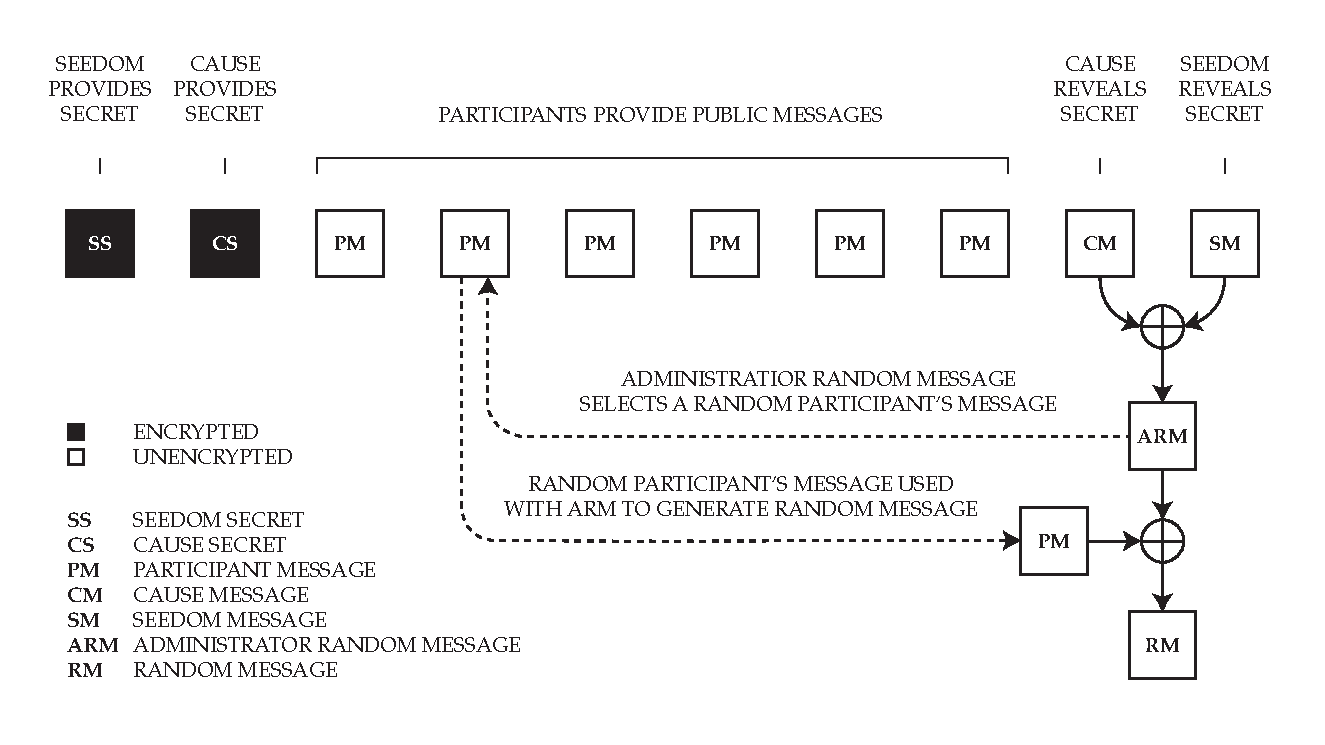
\includegraphics[width=1.0\textwidth]{./graphics/crowd-sourced-random-message-generation.pdf}
\caption{Crowd-sourced random message generation}
\label{figure:crowdsourcedRandomMessageGeneration}
\end{center}
\end{figure}

Many forms of manipulation can occur in the participant-generated portion of the crowd-sourced random message. Manipulation can occur from participants, with access to the entire set of participant messages, and miners, due to miner transaction and block flexibility. The cost of a Seedom entry combined with Ethereum transaction fees is not high enough to deincentivize participants or miners from attempting manipulation.\\\\
However, because the cause and Seedom have seeded additional independent sources of randomization with their revealed messages, such efforts will be in vain. Neither Seedom nor the cause will know of the other's message until revealed. An attacker trying to rig the selection of a participant for reward has to know the secret messages of both Seedom and the cause and has to manipulate the participant-generated portion of the crowd-sourced random message.\\\\
It is a goal of the Seedom team, however, to increase the entropy of the participant-generated randomization effort as much as possible to decentralize the overall random message generation process. Section \ref{sec:increasingTheEntropyOfParticipantGeneratedRandomization} describes future efforts to improve this entropy.

\subsubsection{Participant Selection}

After the crowd-sourced random message generates, it is modded with the number of entries across all participants to determine an index into the total list of entries. During this process, a discrete cumulative density function (CDF) of entries by participant establishes. With this CDF, a binary search is performed to determine and store on-chain the associated participant for this index as the selected participant. Section \ref{sec:improvingParticipantSelectionEfficiency} outlines a more efficient participant selection algorithm for future implementation.

\begin{figure}[H]
\begin{center}
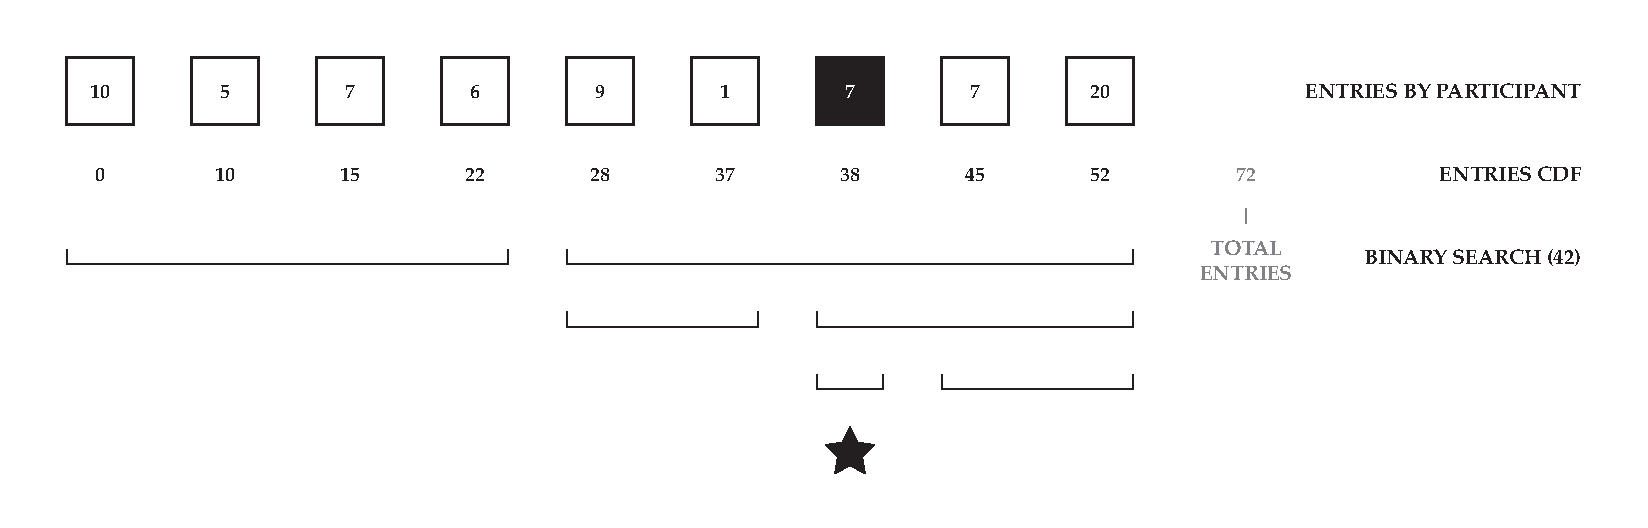
\includegraphics[width=1.0\textwidth]{./graphics/rewarded-participant-selection.pdf}
\caption{Rewarded participant selection for crowd-sourced random message "42"}
\label{figure:participantSelection}
\end{center}
\end{figure}

\subsubsection{Allocation of Ether}

In the same end() function, Ether allocates to the cause, selected participant, and Seedom using the split percentages the fundraiser contract is constructed with, defined in Table \ref{tab:fundraiserDeploymentParameters}. However, Ether is not distributed to any wallets during the end() function to prevent an invalid or malignant address from reverting the Ethereum Virtual Machine (EVM). The withdraw() function in a separate transaction is the only way to pull Ether from the fundraiser contract, for all parties involved.

\subsection{Withdrawing Balances}

After the end() function completes, the cause, selected participant, and Seedom can now withdraw their respective Ether by calling the withdraw() function. These funds are available for withdrawing until the destruct time of the contract. The withdraw() function uses the checks-effects-interactions pattern \cite{7} to avoid a re-entrancy security issue. As a best practice, Seedom recommends that everyone withdraw their funds as soon as possible.

\subsection{Contract Self-destruction}
\label{sec:contractSelfDestruction}

The destruct time for both the fundraiser and polling contracts is set to 3 months from the beginning of a fundraiser. Setting the self-destruct availability time this far into future allows for six more fundraisers to occur and plenty of time for the withdrawal of old contract funds. After the destruct time, Seedom will self-destruct these legacy contracts, and any Ether remaining in them will transfer to Seedom.

\subsection{Fundraiser Cancellation}
\label{sec:fundraiserCancellation}

After the fundraiser contracts are deployed, but before the end() function is called, both the cause and Seedom can cancel the contracts using the cancel() function. Cancellation is a simple process that prevents the fundraiser from proceeding further, refunding all participant entries obtained during the participation and voting phase. Once the cancel() function completes, users may check their balance with the balance() function and withdraw their refund with the withdraw() function. Gas costs are non-refundable.\\\\
After Seedom calls the end() function, early cancellation is impossible; however, if Seedom or the cause fail to reveal their messages before the expire time, the same cancel() function become available to the cause, Seedom, and the entire community. This time-based expiration ensures that every entry is refundable in the improbable event that something catastrophic happens to Seedom, the cause, or both.

\section{Token Sale}
Never.

\section{Future Work}

The fundraiser and polling contracts will be re-deployed for every fundraiser, resulting in new contract addresses for each. Seedom is an agile project continuously improved from user feedback with a release cadence aligned with these deployments. The following are some of the improvements the Seedom team would like to implement going forward.

\subsection{Live Participants Leaderboard}
\label{sec:liveParticipantsLeaderboard}

As more users participate, a live leaderboard will be available that tracks, in descending order, each participant's number of entries. To allow for a leaderboard, an alias will be captured during participation. If a user does not provide an alias for participation, their sending address will be displayed. While not encouraged, participants are free to use this as a way of impromptu advertising. So if Company X wants their name to show within Seedom DAPP, they can buy many entries to display themselves at the top of the leaderboard. This feature requires the implementation of an order statistic tree.

\subsubsection{Order Statistic Tree Participants Storage}

An order statistic tree \cite{5} may replace the dynamic participant storage array in the contract to allow for the live participants leaderboard. A balanced and ordered statistic binary search tree augments the participants mapping, allowing for the efficient rank ordering of participant entries.

\subsection{Enhanced Random Message Generation Security}

Miner manipulation of the crowd-sourced random message generation process requires the Seedom team to adapt the random-generation algorithm in Figure \ref{figure:crowdsourcedRandomMessageGeneration} to stay ahead of potential security issues.

\subsubsection{Increasing the Entropy of Participant-generated Randomization}
\label{sec:increasingTheEntropyOfParticipantGeneratedRandomization}

In the first release of Seedom, participant messages considered in the crowd-sourced random message generation process are XORed in order of time of participation during the participation and voting phase. Randomization of the order of the XORed participant messages using the XOR of the revealed cause and Seedom messages as a seed to this randomization would provide additional entropy and protection against participant and miner manipulation of the final random message.

\subsection{Handling Fund Growth}

As Seedom's participant base grows, our administration fee and participant selection process will evolve.

\subsubsection{Administration Fee Reduction}

The 5\% administration fee is adequate to maintain our DAPP and protect the concept from any legal involvements that may arise. Many laws and organizations span the local and international jurisdictions that might impede the creation of a thoroughly transparent and trustless private global fundraising system of this magnitude. As those concerns dwindle, our administration fee should follow in tandem, at our discretion, to ensure maximum funds for the cause and our community. The Seedom team fully intends to keep the administration fee at or under 5\%.

\subsubsection{Multiple Rewarded Participants}

There is an inherent burden that comes with a sizable influx of funds to any individual. Therefore, as the popularity of Seedom grows, we may introduce, at our discretion, the ability for multiple rewarded participants. Each additionally selected participant might receive more or fewer funds than the previous, or a pool of participants may equally split the reward Ether. However, there is only one benefiting cause per fundraiser.

\subsubsection{Improving Participant Selection Efficiency}
\label{sec:improvingParticipantSelectionEfficiency}

The fundraiser contract currently uses an algorithm similar to roulette wheel selection, while crowd-sourcing random number generation. While acceptably efficient for the initial release, more efficient algorithms exist, such as Vose's alias method \cite{8}. Table \ref{tab:worstCaseAnalysisOfParticipantSelectionAlgorithms} is a worst runtime analysis of these algorithms. The implementation of Vose's method is saved for a future fundraiser contract, due to its slight additional programmatic complexity in Solidity.

\begin{table}[H]
\begin{center}
\begin{tabular}{| l | l | l | l |}
\hline
\textbf{Algorithm} & \textbf{Initialization Time} & \textbf{Generation Time} & \textbf{Memory Usage} \\ \hline
Roulette Wheel Selection & $\Theta(n)$ & $\Theta(log(n))$ & $\Theta(n)$ \\ \hline
Vose's Alias Method & $\Theta(n)$ & $\Theta(1)$ & $\Theta(n)$ \\ \hline
\end{tabular}
\caption{Worst case analysis of participant selection algorithms}
\label{tab:worstCaseAnalysisOfParticipantSelectionAlgorithms}
\end{center}
\end{table}

\subsection{Enhancements to the Polling Contract}
\label{sec:enhancementsToThePollingContract}

The initial release of Seedom uses a proof-of-participation routine that only looks at the currently running fundraiser contract for evidence of user participation. This proof will be enhanced to include all fundraiser contracts that have not self-destructed. Each participant will receive a single vote per fundraiser, independent of the number of entries obtained, allowing engaged Seedom participants an increased effect on the future of Seedom and the causes the team ultimately choose.

\subsection{Giveth Integration}

Seedom is a FUNdraising platform at its core, ensuring Ether is transferred transparently from participants to the organization backing a cause. Giveth is a platform that extends this transparency into the management of this receiving organization, a collection of people referred to as a Decentralized Altruistic Community (DAC). Funds raised from Seedom or through donations are collected and stored in a vault and become available for withdrawal after various milestones complete \cite{11}. Figure \ref{figure:givethIntegration} is a visual explanation of this optional integration.

\begin{figure}[H]
\begin{center}
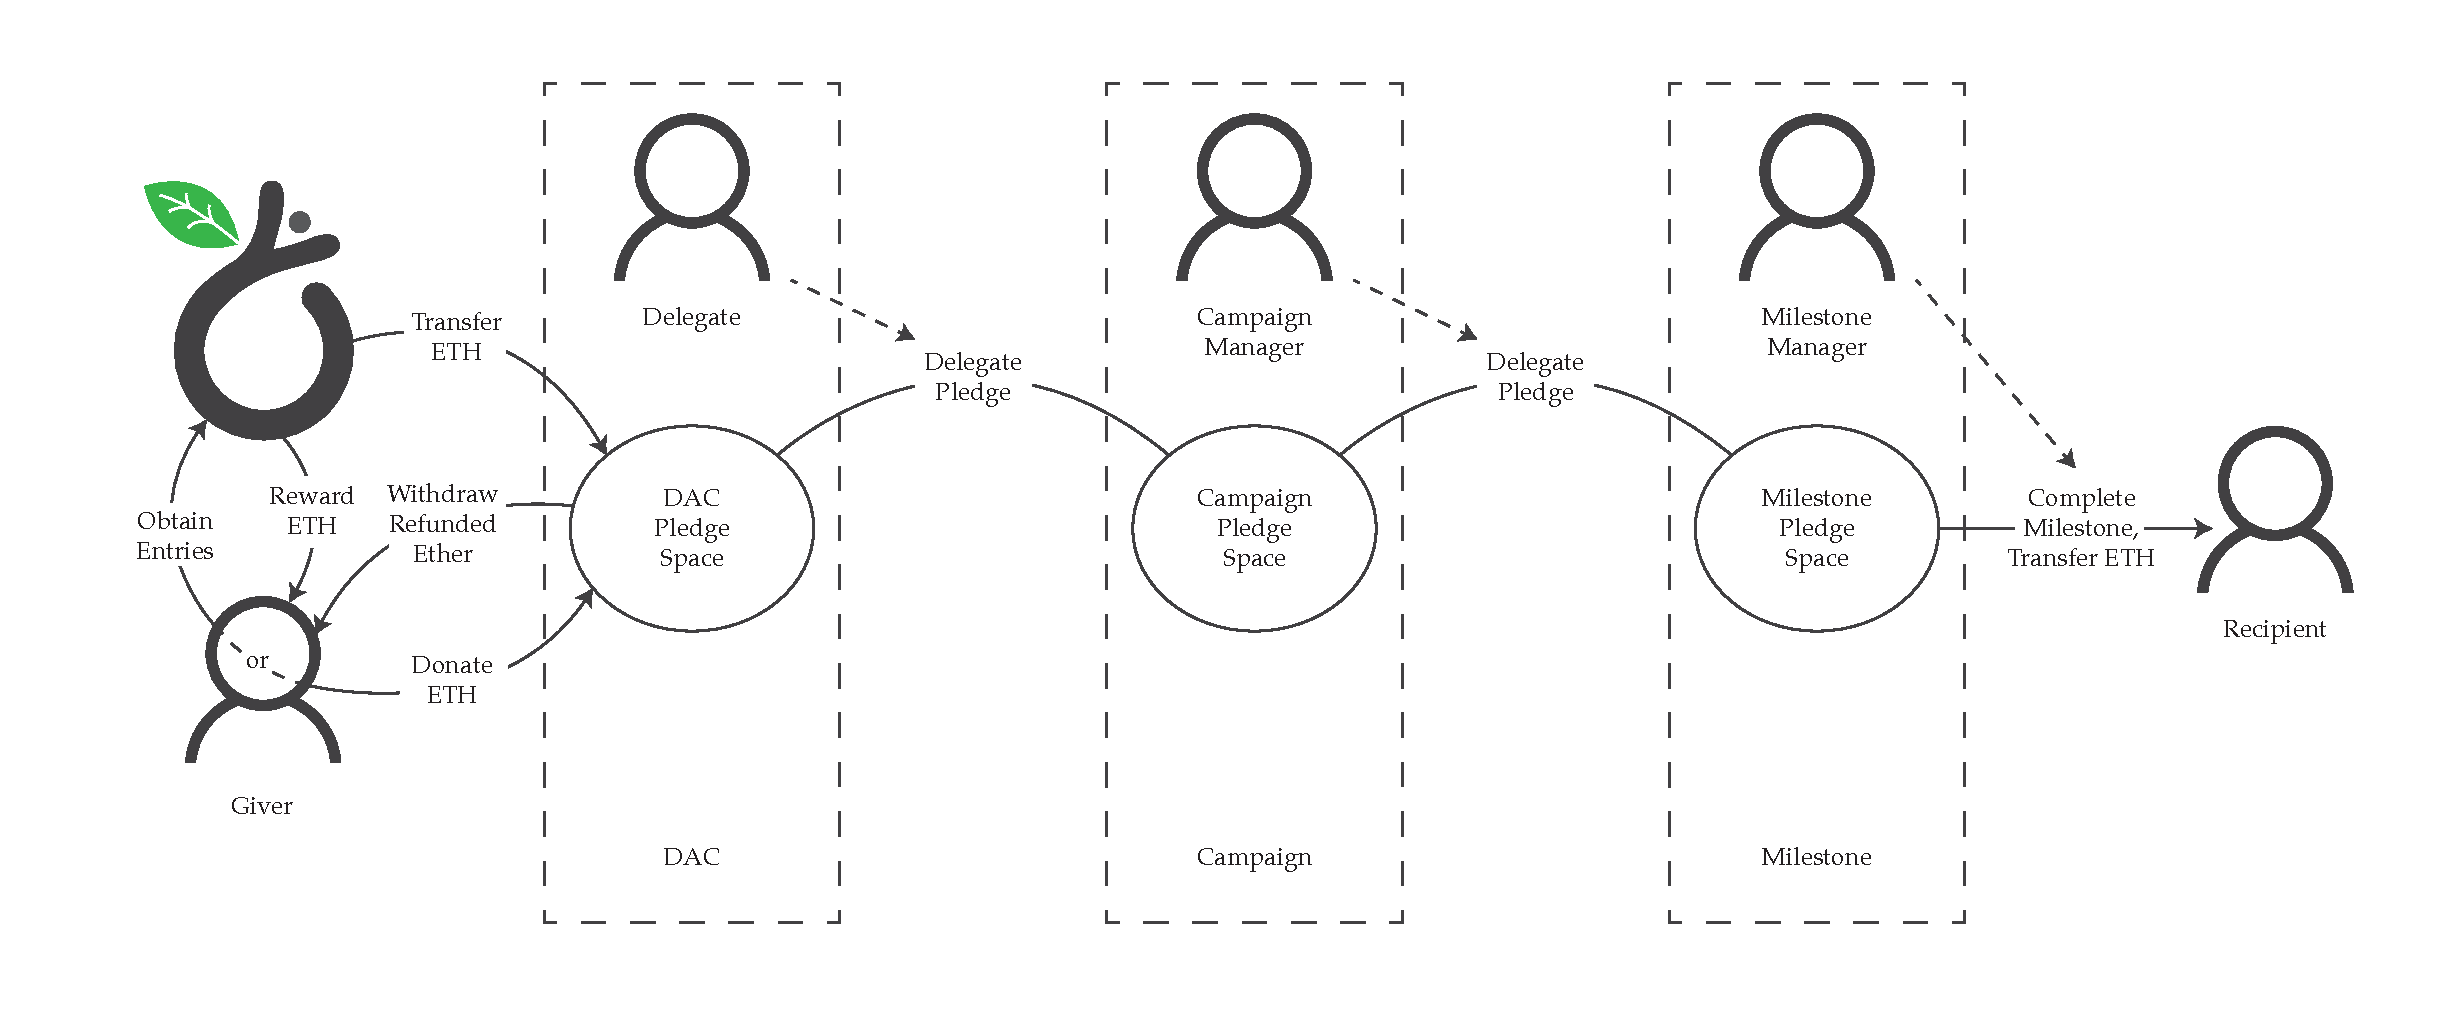
\includegraphics[width=1.0\textwidth]{./graphics/giveth-integration.pdf}
\caption{Giveth integration \cite{11}}
\label{figure:givethIntegration}
\end{center}
\end{figure}

\subsection{Reducing Volatility with Maker Dai}

Most crypto-currencies, including Bitcoin and Ether, can be quite volatile assets. The value of a Bitcoin often experiences sizable fluctuations, rising or falling by as much as 25\% in a single day and 3x in a month \cite{10}. Over the period of a Seedom fundraiser, the price of Ether, compared to fiat currencies such as the U.S. dollar, might change significantly.\\\\
Seedom will likely switch to a more stable crypto-currency, such as Maker Dai, for all smart contract transactions. The Maker platform is decentralized and stabilizes the value of Dai to one U.S. dollar using external market mechanisms and economic incentives. Once generated, Dai transacts in the same manner as any other crypto-currency: it can be freely sent to others, used as payments for goods and services, or held as long-term savings \cite{9}. 

\subsection{Physical Fundraiser and Volunteering Events}

During the recap phase, a physical fundraiser and volunteering event can take place near the headquarters of the benefiting cause to continue bringing awareness, contributions, and volunteers to their cause. This event will be open to the public, and any participant is welcome to attend.\\\\
The rewarded participant or participants will be invited by email if provided to Seedom during participation, to a trip to both the volunteer and fundraising events, wherever they may be in the world. Moreover, Seedom will send some of our team members along to assist the cause with these endeavors.

\section{Team Members}

The Seedom team is diverse, geographically decentralized, and comprised of philanthropic entrepreneurs and enthusiasts from various sectors of the technology industry. The current employers of all team members have no affiliation with Seedom.

\subsubsection{Alexander Groleau}
\begin{minipage}{\textwidth}
\textbf{LinkedIn} https://www.linkedin.com/in/jesse-kuiper-cpa-771a2111\\
\textbf{Role} Founder, Chief Technology Officer (CTO)\\
\end{minipage}

\subsubsection{Eric Thomas}
\begin{minipage}{\textwidth}
\textbf{LinkedIn} https://www.linkedin.com/in/awgneo\\
\textbf{Role} Founder, Chief Information Officer (CIO)\\
\end{minipage}

\subsubsection{Jesse Kuiper}
\begin{minipage}{\textwidth}
\textbf{LinkedIn} https://www.linkedin.com/in/eric-l-m-thomas\\
\textbf{Role} Founder, Chief Executive Officer (CEO)\\
\end{minipage}

\subsubsection{Kyle Graden}
\begin{minipage}{\textwidth}
\textbf{LinkedIn} https://www.linkedin.com/in/kylegraden\\
\textbf{Role} Founder, Chief Marketing Officer (CMO)\\
\end{minipage}

\pagebreak

\printbibliography

\vspace*{\fill}

\begin{flushright}

\pdfcreationdate
\end{flushright}
\end{document}